\chapter{EVENT RECOGNITION}
 In this section we will discuss about the reasons for chosing the convolutional neural network and discuss the features supported by the indigenous neural network that was designed.
 \section{Why CNN~?}
 Covolutional neural networks (CNN) are variant of multiple layer perceptron that are designed by studying the complex arrangement of cells in the cats visual cortex. It fits very well onto the visual recognition domain where we expect the model to handle very high dimensional data, exploit the topology of image or video and be invariant to small translation and illumination changes. CNN leverage following concepts,
\subsubsection{Local Connectivity}
It exploits the spatially local correlation by enforcing local connectivity pattern between neurons of adjacent layers. In other words, every hidden units is only sensitive to a small block in  the visual field, called receptive field. This drastically reduces the number of connections between input and hidden layer, following which diminishes the number of parameters needed to train the model.
\subsubsection{Shared Filters}
The hidden units are associated to the receptive field by filters which are shared within a feature map. These filters tries to capture edge like patterns within the receptive field. Additionally, sharing filters increases learning efficiency by greatly reducing the number of free parameters to be learned. Apart from reducing parameters, they extract the same feature at every position, which makes every feature map to be equi-variant to any changes in the input. The shared filters are associated to the receptive field by a dot product operation which can be expressed as a discrete convolution operation.
\subsubsection{Pooling/Sub-sampling Hidden Units}
According to this concept, we try to pool the hidden in non-overlapping neighborhood. Among the techniques average and max pooling, max pooling has been commonly used as it provides local translation in-variance. Pooling also reduces inputs to next layer of feature extraction, thus allowing us to have many more feature maps. All feature maps in latter layer extracts coarser features.\par
All these concepts enable CNN to achieve better generalization in the vision problems. We stack multiple such layers to achieve better responsiveness to larger visual field. \section{Python-DNN Toolkit}
All these concepts enable CNN to achieve better generalization in the vision problems. We stack multiple such layers to achieve better responsiveness to larger visual field.
\subsection{Implementation}
Implementation of CNN is done in python using numerical computation library named \textit{Theano}. It provides platform to run efficiently in CPU and GPU architecture. Following are some key features of our implementation
\begin{itemize}
	\item  Allows easy configuration of the model, configurations are organized in JSON format thus makes the configuration legible to humans.
	\item Supports several types of data readers/writers.
	\item Enables us to dump CNN features for their use in other applications.
	\item Facilitates in loading pre-trained model and dumping the trained model.
	\item Supports two and three dimensional convolutional models.
	\item Run efficiently in CPU and GPU architectures.
	
\end{itemize}
Our implementation is publicly made available in github\footnote{\url{https://github.com/IITM-DONLAB/python-dnn}}. Architecture of the indigenous DNN toolkit is shown on \ref{fig:architecture}.Sample configurations for some well known dataset like MNIST and CIFAR are also made available with it.
\begin{figure}[htpb]
   \begin{center}
	    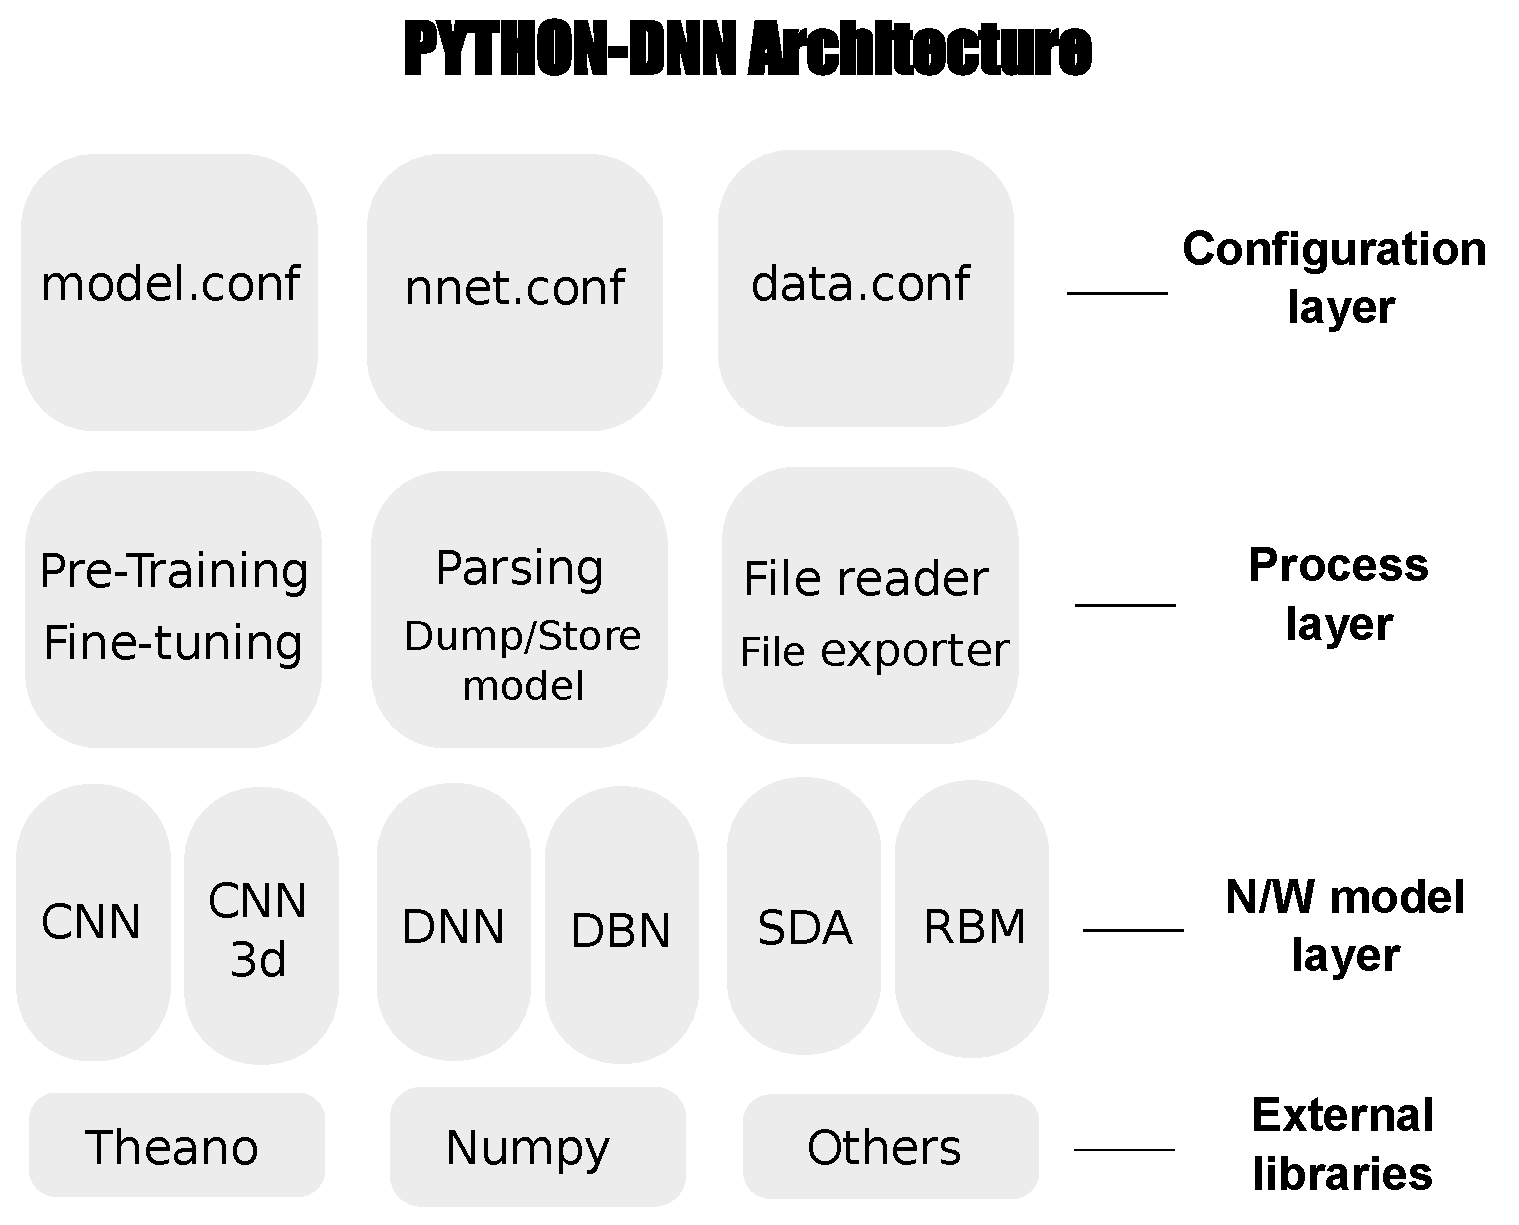
\includegraphics[width=0.75\textwidth]{snaps/architecture.eps}     
     \caption {Python-DNN Architecture}
	 \label{fig:architecture}
   \end{center}
 \end{figure}